\chapter{METHODOLOGY}
\label{sec:chap3_metodologi}

\section*{ }
This section describes our proposed method for pose estimation-based classification of elderly exercise activities using deep learning. We begin our work by determining the types of exercises that the elderly can do to address health issues in old age. One of the challenges of our work is the limited dataset available. So in collecting datasets, we created new datasets according to the predetermined dataset classes. The dataset we have is then subjected to preprocessing and keypoint extraction. The keypoint extraction set is trained using deep learning architecture to produce the desired model. The results of this model are then subjected to evaluation metrics to review our model. Figure \ref{fig:blokdiagram} provides a brief summary of the proposed method.

\begin{figure}[h!]
	\centering
	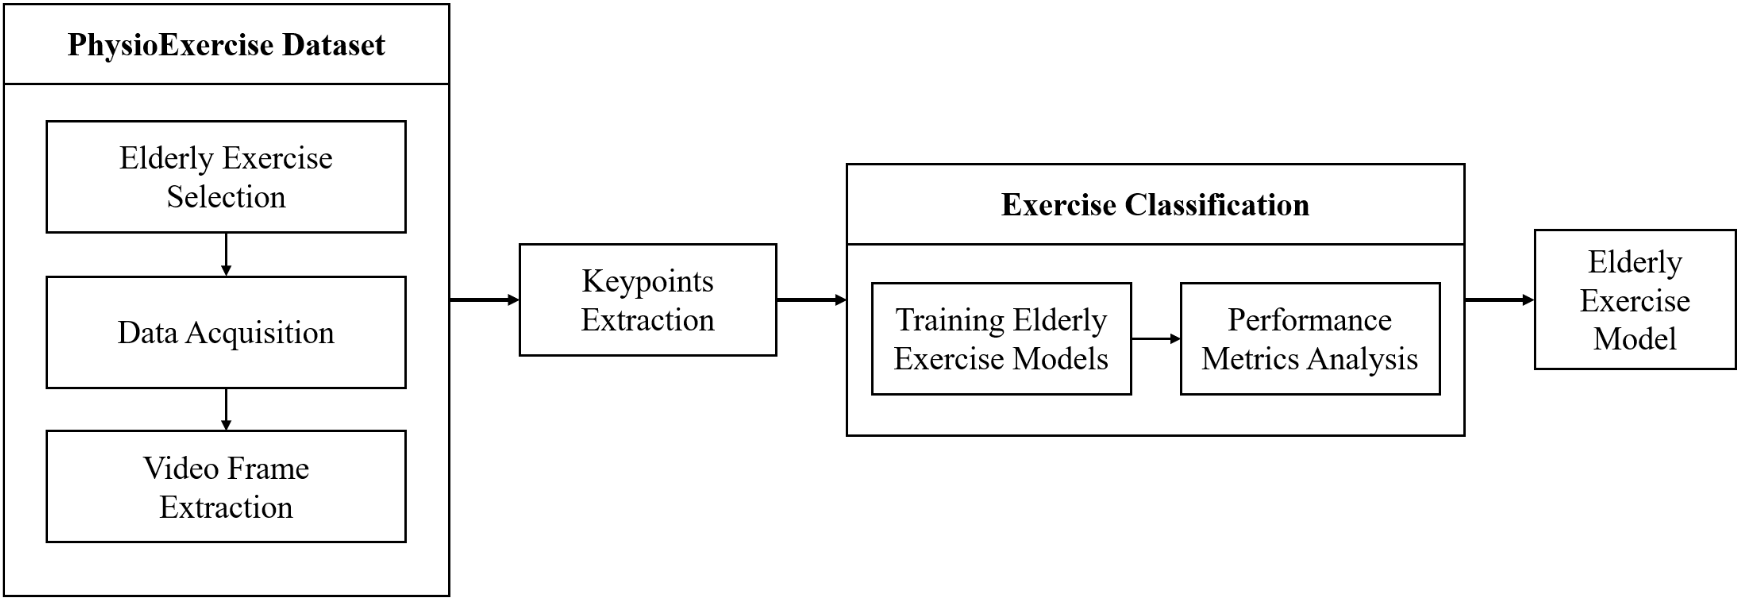
\includegraphics[width=\linewidth]{bab3/ar_BlockDiagram4.png}
	\caption{Research Block Diagram}
	\label{fig:blokdiagram}
\end{figure}

\section{PhysioExercise Dataset}
\label{sec3:physioexercise_dataset}
Exercise performed by the elderly is different from exercise performed in general. Since the elderly have special issues regarding their health, the exercises given must be adapted to their conditions. There are not many exercise datasets for the elderly. Therefore, this section explains the process of creating a dataset that is suitable for elderly exercise activities.
% Exercise yang dilakukan oleh elderly berbeda dengan exercise yang dilakukan secara umum. Sejak elderly memiliki isu-isu khusus mengenai kesehatannya, exercise yang diberikan harus disesuaikan dengan kondisi mereka. Tidak banyak dataset exercise untuk elderly. Oleh karena itu, bagian ini menjelaskan proses pembuatan dataset yang sesuai untuk aktifitas exercise elderly.


\subsection{Elderly Exercise Selection}
\label{subsec3:elderly_exercise_selection}
As a first step in our work, we had to determine the types of exercises for the elderly. Most human activity recognition, especially for the elderly, revolves around daily activities such as standing, sitting, lying down, eating, opening doors, etc. \cite{elderly2, elderly1}. Exercises performed for the elderly must be more selective and careful due to their physical condition. Therefore, it must be consulted with physiotheraphists first. In addition, the exercises that will be categorized are the types of exercises that can be done alone and at home. One example of exercises that fit the criteria is in \cite{dataset1}. The work shows physiotherapy activities for the elderly that can be done at home. In addition, the exercises are specialized based on health issues that are common to the elderly physique.

\subsection{Dataset Acquisition}
\label{subsec3:dataset_acquisition}
We made adjustments to the dataset we used. The dataset used is a collection of physiotherapy exercise videos for the elderly based on predetermined classes. The videos were taken in our laboratory and some were taken in the home environment. Since the utilization of physiotherapy exercises is done at home independently, the use of mobile phone cameras is one of the effective solutions. Therefore, we used mobile phone cameras as input for dataset capture. The camera specifications used in this work are 64 MP, 26mm focal length, f/1.8 aperture lens, 0.8µm pixel size, and 1/1.7" sensor size. The dataset was captured in the form of a 1080p resolution video. There is 30 frames per second in the video.

We varied the angle of the video capture. We placed the camera at 3 angles, i.e., straight ahead, \ang{30} angle relative to the left, and \ang{30} angle relative to the right. In addition to the camera angle, we also gave people a variety of angles. We apply various orientations of the person's position to the camera. This aims to enrich our dataset. However, we limit these orientations to the possible positions of the elderly in performing physiotherapy exercises.

\subsection{Video Frame Extraction}
\label{subsec3:VideoExtraction}

The acquired data is a collection of exercise activity videos. This data is organized in each folder according to the predefined class classification. We perform data preprocessing after we have collected all the required video datasets. We divided each video into 100 images. These images are sequences of physiotherapy exercise activities for each class that will have their keypoint values extracted. We have selected the videos so that they still have a high diversity value for each class.
% Data yang telah diakuisisi merupakan kumpulan video aktifitas latihan. Data ini diorganisir dalam masing-masing folder sesuai dengan klasifikasi kelas yang telah ditentukan sebelumnya. Kami melakukan prapemrosesan data setelah kami mengumpulkan semua set data video yang diperlukan. Kami membagi setiap video menjadi 100 gambar. Gambar-gambar ini adalah urutan kegiatan latihan fisioterapi untuk setiap kelas yang akan diekstraksi nilai keypoint-nya. Kami telah memilih video-video tersebut sehingga masih memiliki nilai keragaman yang tinggi untuk setiap kelas.

\section{Keypoint Extraction}
\label{sec:keypoint_extraction}

In this stage, we focus on the keypoint feature extraction process which is crucial for human motion analysis in the context of exercise activity classification for the elderly. This keypoint extraction is performed by utilizing the MediaPipe framework, a solution developed by Google to enable real-time and accurate human pose estimation. MediaPipe facilitates the extraction of keypoint coordinates by using machine learning models that have been trained on large and diverse datasets, enabling efficient human body position detection.
% Dalam tahap ini, kami fokus pada proses ekstraksi fitur keypoint yang krusial untuk analisis gerak manusia dalam konteks klasifikasi aktivitas latihan untuk elderly. Ekstraksi keypoint ini dilakukan dengan memanfaatkan framework MediaPipe, sebuah solusi yang dikembangkan oleh Google untuk memungkinkan estimasi pose manusia secara real-time dan akurat \cite{BlazePose}. MediaPipe memfasilitasi ekstraksi koordinat keypoint dengan menggunakan model pembelajaran mesin yang telah terlatih pada dataset yang luas dan beragam, memungkinkan deteksi posisi tubuh manusia secara efisien.

The extraction process begins with the receipt of video frames as input, where each frame first undergoes pre-processing to ensure that the incoming data is in optimal condition for analysis. Normalization is performed on the obtained pixel coordinates, converting them to a scale that is consistent and independent of the original dimensions of the image, thus enabling accurate comparisons among different sources and image resolutions. Coordinate normalization is done following equations \eqref{eq: pers.1} and \eqref{eq: pers.2}.
% Proses ekstraksi dimulai dengan penerimaan frame video sebagai input, di mana setiap frame pertama-tama mengalami pra-pemrosesan untuk memastikan bahwa data yang masuk dalam kondisi optimal untuk analisis. Normalisasi dilakukan pada koordinat piksel yang diperoleh, mengkonversi mereka ke skala yang konsisten dan independen dari dimensi asli gambar, sehingga memungkinkan komparasi yang akurat di antara berbagai sumber dan resolusi gambar.

\begin{equation}\label{eq: pers.1}
	(x',y') = \left(\frac{x}{widht},\frac{y}{height}\right)
\end{equation}

Width and height refer to image dimensions. Equation \eqref{eq: pers.2} refers to depth normalization (z-depth). The minimun and maximum depths represented by \(z\textsubscript{min}\) and \(z\textsubscript{max}\) are detected within the frame or a preset range.

\begin{equation}\label{eq: pers.2}
	z' = \frac{z-z_{min}}{z_{max}-z_{min}}
\end{equation}

After preprocessing, the frames are processed using MediaPipe's pose estimation model that uses a Convolutional Neural Network (CNN) architecture. This model effectively identifies and tracks 33 keypoints located in key areas of the human body, such as the head, shoulders, elbows, wrists, hips, knees and ankles. Each keypoint is detected with \((x, y, z)\) coordinates and comes with a confidence score that indicates the accuracy of the detection.Since Mediapipe Pose Estimation has 33 keypoints, we utilize all of them in our work. We perform indexing for each keypoint. Indexing keypoints follows the equation \ref{eq: pers.3}.
% Setelah pra-pemrosesan, frame tersebut diproses menggunakan model pose estimation dari MediaPipe yang menggunakan arsitektur Convolutional Neural Network (CNN). Model ini secara efektif mengidentifikasi dan melacak 33 keypoint yang berlokasi di area penting tubuh manusia, seperti kepala, bahu, siku, pergelangan tangan, pinggul, lutut, dan pergelangan kaki. Setiap keypoint dideteksi dengan koordinat x,y,z dan dilengkapi dengan skor kepercayaan yang mengindikasikan keakuratan deteksi tersebut.

\begin{equation}\label{eq: pers.3}
	KP = {kp_0, kp_1,..., kp_{32}}
\end{equation}

Where each \(kp\textsubscript{i}\) corresponds to a specific part like the nose, left eye inner, right eye, etc.

The keypoints in this work are represented as vectors. The vector in Mediapipe Pose Estimation consists of keypoint \(kp\textsubscript{i}\) 3-axis coordinates \((x, y, z)\) and confidence value \(c\). Thus, the vector \(V\) for a single image could be:
% $(x, y, z)$

\begin{equation}\label{eq: pers.4}
	V = \left[\left(x_0, y_0, z_0, c\right), \left(x_1, y_1, z_1, c\right),...,\left(x_{32}, y_{32}, z_{32}, c\right)\right]
\end{equation}

Each frame that has gone through pose estimation is then stored in an array file in '.npy' format. In this storage file, there are two lists, namely sequences and labels. The sequences list will store the sequential data, containing the keypoints feature information that will be used for training. The labels list contains the labels associated with the sequences data, which gives the class information of each data. In a data set, there are 100 images that represent the number of windows in the data. Each window has keypoint coordinate data according to equation \ref{eq: pers.4}. This \(V\) vector becomes the feature used for training data. One window will have an array of size 132 because 33 keypoints have 4 vector values. So, the data format used in this study is:
% Setiap frame yang telah melalui estimasi pose, kemudian disimpan dalam sebuah file array dalam format '.npy'. Di dalam file penyimpanan ini terdapat dua list, yaitu sequences dan labels. List sequences akan menyimpan data sekuensial, berisikan informas fitur keypoints yang akan digunakan untuk pelatihan. List labels berisikan label yang terkait dengan data sekuensial di mana memberikan informasi kelas dari masing-masing data. Dalam sebuah set data, terdapat 100 citra yang merepresentasikan jumlah window satu data. Setiap window memiliki data koordinat keypoint sesuai dengan persamaan \ref{eq: pers.4}. Vektor \(V\) ini menjadi fitur yang digunakan untuk data pelatihan. Satu window akan memiliki array dengan ukuran 132 karena 33 titik kunci memiliki 4 nilai vektor. Jadi, format data yang digunakan pada penelitian ini adalah:

\begin{equation}
	\label{eq: pers.5}
	X = (nData, nWindow, nFeatures)
\end{equation}

\begin{equation}
	\label{eq: pers.6}
	y = (nData, nClass)
\end{equation}

where X stores the sequential data of the dataset and y is the label for each data. nData is the total amount of data used in this dataset. It indicates how many sequences we have. nWindow represents the sequence length or number of frames in each data. In this case nWindow is 100. nFeatures is the number of features in a data frame. It indicates how many values are described in each frame. In a pose estimation using the Mediapipe framework, there are 132 feature data extracted. nClass is the number of classes that will divide each data following the training activity label. This number is predefined as 9 exercise activity classes.
% di mana X menyimpan data sekuensial dataset dan y merupakan label untuk setiap data. nData merupakan jumlah total data yang digunakan dalam dataset ini. Bagian ini menunjukkan seberapa banyak sequences yang dimiliki. nWindow merepresentasikan panjang urutan atau jumlah frame dalam setiap data. Dalam hal ini nWindow berjumlahh 100. nFeatures merupakan jumlah fitur dalam sebuah data frame. Ini menunjukkan berapa banyak nilai yang dijelaskan dalam setiap frame. Pada sebuah estimasi pose menggunakan framework Mediapipe, terdapat 132 data fitur yang diekstraksi. nClass adalah jumlah kelas yang akan membagi setiap data mengikuti label aktifitas latihan. Jumlah ini telah ditentukan sebelumnya sebanyak 9 kelas aktitias latihan. 

In the training process, the data sequences and labels of the entire dataset are combined into one file with the '.npz' format. This file format is a format used to store multiple arrays in one file. An '.npz' file is a zip archive containing multiple '.npy' files where each array is stored as a separate '.npy' file within the archive. This format makes it possible to store arrays in a larger form.
% Untuk memudahkan proses pelatihan, data sequences dan labels seluruh dataset digabungkan menjadi satu ke dalam file dengan format '.npz'. Format file ini adalah format yang digunakan untuk menyimpan beberapa array dalam satu file. File '.npz' adalah arsip zip berisikan beberapa file '.npy' di mana setiap array disimpan sebagai file '.npy' terpisah di dalam arsip. Format ini memungkinkan untuk menyimpan array dalam bentuk yang lebih besar. 

\section{Training Model}
\label{sec3: training_model}
We trained on a laptop with an AMD Ryzen 5900HX with an integrated graphics card, NVIDIA RTX 3050 GPU support, 4 GB of VRAM, and DDR4 16 GB of RAM. The parameters used in this training apply to all models used. Our system is built in a Jupyter Notebook container with Python and the Tensorflow framework. The dataset training is done over 100 epochs. We used 80\% data for data training and 20\% data for data validation. Details of the parameters used can be seen in Table \ref{tab:hyperparameters}.

\begin{table}[h!]
	\centering
	\caption{Training model hyperparameter configuration.}
	\label{tab:hyperparameters}
	\begin{tabular}{|l|l|}
		\hline
		Epoch            & 100                      \\ \hline
		Batch Size       & 16                       \\ \hline
		Learning Rate    & 0.001                    \\ \hline
		Optimizer        & Adam                     \\ \hline
		Loss             & Categorical Crossentropy \\ \hline
		Activation Layer & ReLU, Softmax            \\ \hline
		Class            & 9                        \\ \hline
	\end{tabular}
\end{table}

\subsection{CNN Architecture}

The architecture shown in figure \ref{fig:CNNArch} is a one-dimensional Convolutional Neural Network (CNN) model (Conv1D). Conv1D is chosen because the data used is sequential data or time-based data. The data form used is \(X = (nData, nWindow, nFeatures)\). Each sample is a temporal sequence of features taken from each frame. The features used are keypoints extracted from the pose estimation. Conv1D is simpler compared to other number of dimensions because it only works along one dimension, reducing the amount of computation, and parameters to be optimized. Conv1D also has good dimensionality reduction and local pattern detection capabilities. This relates to the way a model reduces data complexity by extracting important features from temporal sequences and finding relationships between keypoints in short time sequences.
% Arsitektur yang ditunjukkan pada gambar \ref{fig:CNNArch} adalah model Convolutional Neural Network (CNN) satu dimensi (Conv1D). Conv1D dipilih karena data yang digunakan adalah data sekuensial atau data berbasis waktu. Bentuk data yang digunakan adalah \(X = (nData, nWindow, nFeatures)\). Setiap sampel adalah urutan temporal dari fitur-fitur yang diambil dari setiap frame. Fitur yang digunakan adalah keypoint hasil ekstraksi dari pose estimasi. Conv1D lebih sederhana dibandingkan dengan jumlah dimensi lainnya karena hanya bekerja sepanjang satu dimensi, mengurangi jumlah komputasi, dan parameter yang harus dioptimalkan. Conv1D juga memiliki kemampuan yang baik dalam mereduksi dimensi dan mendeteksi pola lokal. Hal ini berhubungan dengan cara sebuah model mengurangi kompleksitas data dengan mengekstraksi fitur penting dari urutan temporal dan menemukan hubungan antara keypoint dalam urutan waktu yang singkat. 

\begin{figure}[h!]
	\centering
	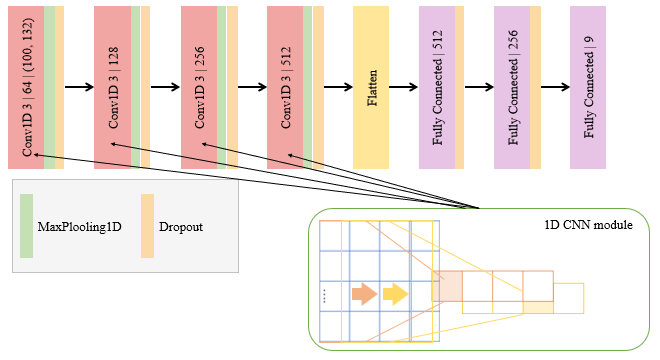
\includegraphics[width=\linewidth]{bab3/ar_CNNArch.png}
	\caption{Architecture of CNN that used in this research.}
	\label{fig:CNNArch}
\end{figure}

The model consists of several main components. First, there are four 1D convolution layers (Conv1D) with a kernel of size 3, which have 64, 128, 256, and twice 512 filters, respectively. These layers are responsible for extracting features from the input data. After each convolution layer, there is a MaxPooling1D layer that is used to reduce the dimensionality of the data and capture the main features, helping in reducing the data size and computation. In addition, multiple convolution layers are followed by a dropout layer to prevent overfitting by randomly disabling a number of units in the network during training. The output of the convolution and pooling layers is then flattened using the Flatten layer, turning the data into a 1D vector that can be fed to the fully connected layer. There are three fully connected layers in this architecture, with 512, 256, and 9 units respectively, where the last layer is typically used as the output layer for classification into 9 classes.
% Model ini terdiri dari beberapa komponen utama. Pertama, terdapat lima lapisan konvolusi 1D (Conv1D) dengan kernel ukuran 3, yang berturut-turut memiliki 64, 128, 256, dan dua kali 512 filter. Lapisan-lapisan ini bertugas mengekstrak fitur dari data input. Setelah setiap lapisan konvolusi, terdapat lapisan MaxPooling1D yang digunakan untuk mengurangi dimensi data dan menangkap fitur utama, membantu dalam mengurangi ukuran data dan komputasi. Selain itu, beberapa lapisan konvolusi diikuti oleh lapisan dropout untuk mencegah overfitting dengan secara acak menonaktifkan sejumlah unit dalam jaringan selama pelatihan. Output dari lapisan konvolusi dan pooling kemudian diratakan menggunakan lapisan Flatten, mengubah data menjadi vektor 1D yang dapat diumpankan ke lapisan fully connected. Terdapat tiga lapisan fully connected dalam arsitektur ini, dengan masing-masing 512, 256, dan 9 unit, di mana lapisan terakhir biasanya digunakan sebagai lapisan output untuk klasifikasi ke dalam 9 kelas.

Overall, this architecture is designed to process sequential data by extracting features through a convolution layer, reducing dimensionality by pooling, preventing overfitting with dropout, and performing classification through a fully connected layer. This combination makes the 1D CNN model very suitable for tasks such as signal analysis, text processing, or other sequential data.
% Secara keseluruhan, arsitektur ini dirancang untuk mengolah data sekuensial dengan cara mengekstrak fitur melalui lapisan konvolusi, mengurangi dimensi dengan pooling, mencegah overfitting dengan dropout, dan melakukan klasifikasi melalui lapisan fully connected. Kombinasi ini membuat model 1D CNN sangat cocok untuk tugas-tugas seperti analisis sinyal, pemrosesan teks, atau data sekuensial lainnya.


\subsection{LSTM Architecture}

Another architecture used is the LSTM. This architecture is a further development of the traditional RNN. LSTMs address the traditional RNN problems of vanishing gradient and long-term dependencies. LSTMs are able to remember important information for a longer period of time than traditional RNNs. The data used in this research is time series data with long temporal patterns, making LSTM suitable for this dataset.
% Arsitektur lain yang digunakan adalah LSTM. Arsitektur ini merupakan pengembangan lebih lanjut dari RNN tradisional. LSTM menangani masalah RNN tradisional terkait vanishing gradient dan long-term dependencies. LSTM mampu mengingat informasi penting untuk jangka waktu lebih panjang dibanding RNN biasa. Data yang digunakan pada penelitian ini merupakan data time series dengan pola temporal panjang, menjadikan LSTM cocok untuk dataset ini. 

\begin{figure}[h!]
	\centering
	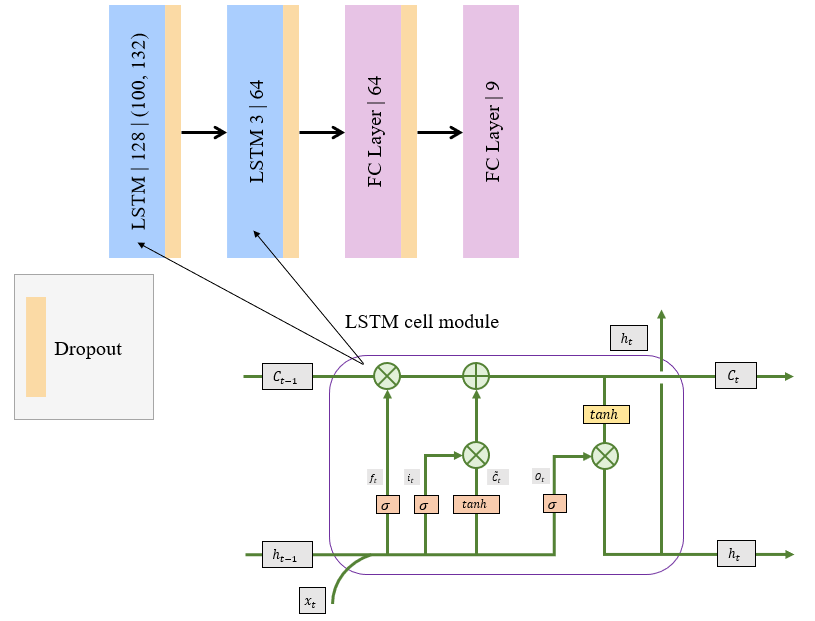
\includegraphics[width=\linewidth]{bab3/ar_LSTMArch.png}
	\caption{Architecture of LSTM that used in this research.}
	\label{fig:LSTMArch}
\end{figure}

The architecture shown in figure \ref{fig:LSTMArch} is a Long Short-Term Memory (LSTM) model used for processing sequential or time-based data. This model consists of several main components. First, there are two LSTM layers. The first LSTM layer has 128 units and accepts inputs with dimensions (100, 132), followed by a dropout layer to prevent overfitting by randomly disabling a number of units in the network during training. The second LSTM layer has 64 units and is also followed by a dropout layer. This LSTM layer is used to capture long-term dependencies in sequential data.
% Arsitektur yang ditunjukkan pada gambar \ref{fig:LSTMArch} adalah model Long Short-Term Memory (LSTM) yang digunakan untuk memproses data sekuensial atau data berbasis waktu. Model ini terdiri dari beberapa komponen utama. Pertama, terdapat dua lapisan LSTM. Lapisan LSTM pertama memiliki 128 unit dan menerima input dengan dimensi (100, 132), diikuti oleh lapisan dropout untuk mencegah overfitting dengan secara acak menonaktifkan sejumlah unit dalam jaringan selama pelatihan. Lapisan LSTM kedua memiliki 64 unit dan juga diikuti oleh lapisan dropout. Lapisan LSTM ini digunakan untuk menangkap dependensi jangka panjang dalam data sekuensial.

After the LSTM layer, the output is flattened and fed to two fully connected (FC) layers. The first fully connected layer has 64 units, while the second fully connected layer has 9 units, which is usually used as the output layer for classification into 9 classes. The diagram on the bottom right shows the LSTM cell module in detail, which illustrates the internal mechanism of the LSTM cell including the input gate (\(i_t\)), forgetting gate (\(f_t\)), and output gate (\(o_t\)), as well as how the state cells (\(C_t\)) are updated through sigmoid operation (\(\sigma\)) and tanh activation function.
% Setelah lapisan LSTM, output diratakan dan diumpankan ke dua lapisan fully connected (FC). Lapisan fully connected pertama memiliki 64 unit, sementara lapisan fully connected kedua memiliki 9 unit, yang biasanya digunakan sebagai lapisan output untuk klasifikasi ke dalam 9 kelas. Diagram di kanan bawah menunjukkan modul sel LSTM secara detail, yang menggambarkan mekanisme internal dari sel LSTM termasuk gerbang input (\(i_t\)), gerbang melupakan (\(f_t\)), dan gerbang output (\(o_t\)), serta bagaimana sel-sel status (\(C_t\)) diperbarui melalui operasi sigmoid (\(\sigma\)) dan fungsi aktivasi tanh. 

The architecture's overall goal is to handle and evaluate sequential data by utilizing the fully connected layer to do classification, the LSTM layer to capture temporal information, and dropout to minimize overfitting. Because of this combination, the LSTM model performs exceptionally well in applications like signal processing, time series prediction, and text analysis.
% Secara keseluruhan, arsitektur ini dirancang untuk memproses dan menganalisis data sekuensial dengan menangkap informasi temporal menggunakan lapisan LSTM, mencegah overfitting dengan dropout, dan melakukan klasifikasi melalui lapisan fully connected. Kombinasi ini membuat model LSTM sangat efektif dalam tugas-tugas seperti analisis teks, prediksi deret waktu, dan pemrosesan sinyal.

\subsection{CNN-LSTM Architecture}
\begin{figure}[h!]
	\centering
	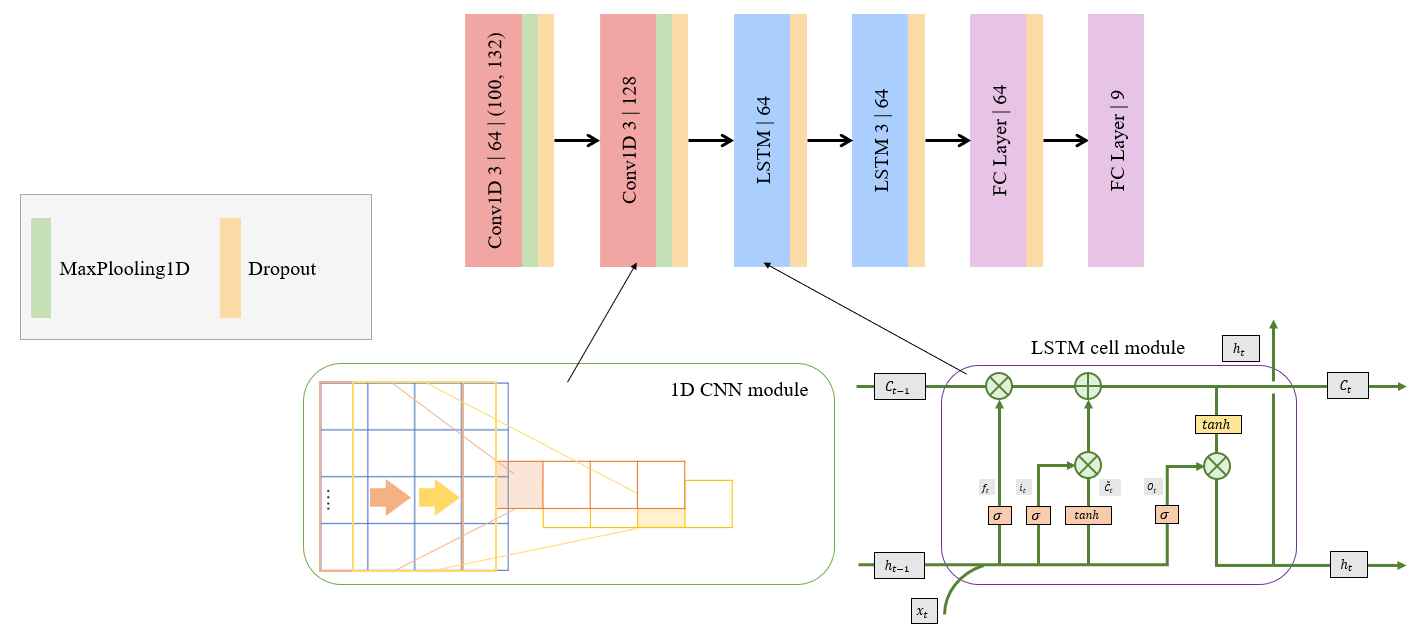
\includegraphics[width=\linewidth]{bab3/ar_CNNLSTMArch.png}
	\caption{Architecture of CNN-LSTM that used in this research.}
	\label{fig:CNNLSTMArch}
\end{figure}

Our proposed CNN-LSTM architecture starts with two consecutive one-dimensional convolution (Conv1D) layers, each followed by a one-dimensional max pooling (MaxPooling1D) layer. The first Conv1D layer has the objective of capturing local features of the input sequence, with the convolution kernel applying a non-linear filter on a subset of the data. After each convolution layer, the MaxPooling1D layer is used to reduce the output dimension and control overfitting by taking the maximum value of a small subset of the convolution layer output. Next, the architecture continues with two Long Short-Term Memory (LSTM) layers followed by a dropout layer. The first LSTM layer serves to capture temporal dependencies in the data sequence, while the subsequent dropout layer helps reduce overfitting by randomly disabling units during training. The second LSTM layer deepens the model's understanding of complex sequence patterns, followed by another dropout layer for additional regulation. Then, the model ends with two Dense layers, each of which is followed by a dropout layer. The first Dense layer with ReLU activation function serves to combine the learned features and apply them to a lower output dimension. The last dropout layer ensures that the model still generalizes well to data that has never been seen. Finally, a second Dense layer with a softmax activation function is used to generate the final prediction that represents the probability of each possible class. The output of this model is a model that can classify 9 classes of elderly exercise activities.

\subsection{Deep CNN-LSTM Architecture}

\begin{figure}[h!]
	\centering
	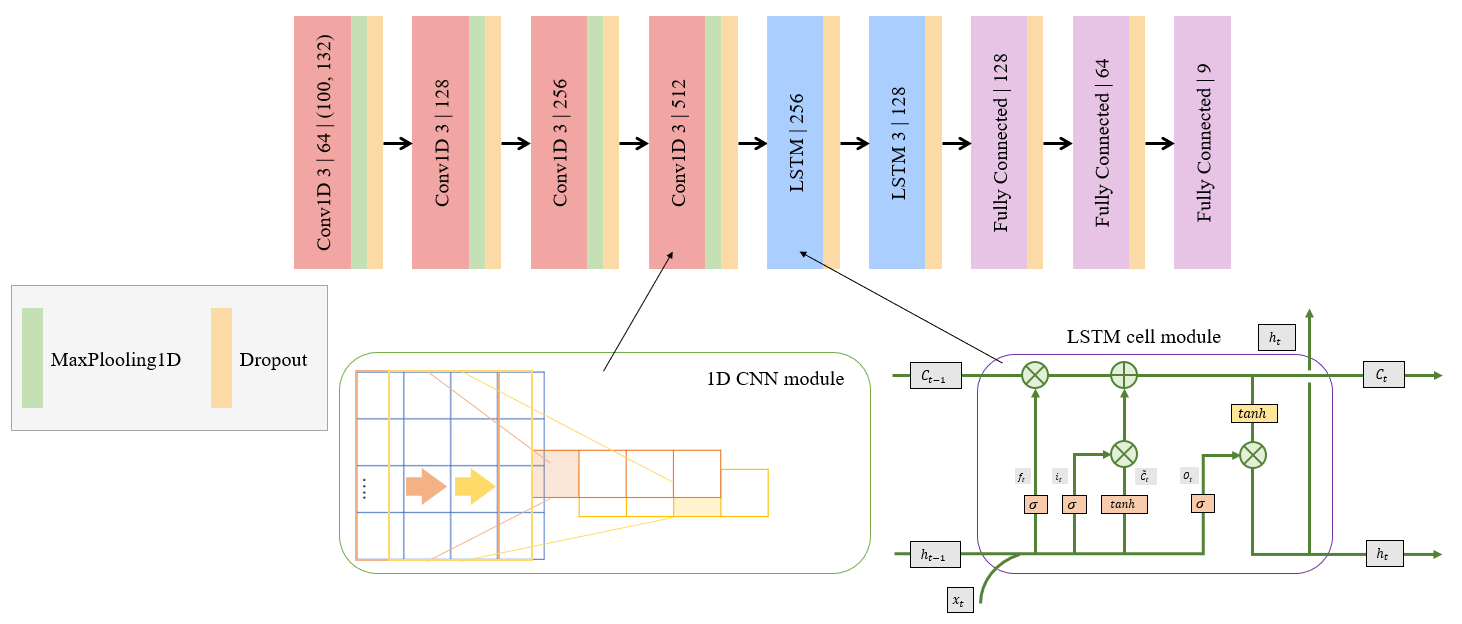
\includegraphics[width=\linewidth]{bab3/ar_DeepCNNLSTMArch.png}
	\caption{Architecture of Deep CNN-LSTM that used in this research.}
	\label{fig:DeepCNNLSTMArch}
\end{figure}

The architecture shown in figure \ref{fig:DeepCNNLSTMArch} is a combination of a one-dimensional Convolutional Neural Network (CNN) (1D CNN) and Long Short-Term Memory (LSTM) model designed to process sequential or time-based data, such as signals or text data. The model consists of several main components that work sequentially.
% Arsitektur yang ditunjukkan pada gambar \ref{fig:DeepCNNLSTMArch} adalah kombinasi dari model Convolutional Neural Network (CNN) satu dimensi (1D CNN) dan Long Short-Term Memory (LSTM) yang dirancang untuk memproses data sekuensial atau data berbasis waktu, seperti sinyal atau data teks. Model ini terdiri dari beberapa komponen utama yang bekerja secara berurutan.

The first layer consists of several 1D convolution layers (Conv1D) with a size 3 kernel. The first convolution layer takes input with dimensions (100, 132) and has 64 filters. A Conv1D layer with 128 filters is next, then a layer with 256 filters, and two layers with 512 filters apiece. After each of these convolution layers, there is a dropout layer to avoid overfitting and a MaxPooling1D layer to reduce the dimensionality of the data and capture important characteristics.
% Pertama, terdapat beberapa lapisan konvolusi 1D (Conv1D) dengan kernel ukuran 3. Lapisan konvolusi pertama memiliki 64 filter dan menerima input dengan dimensi (100, 132). Selanjutnya, terdapat lapisan Conv1D dengan 128 filter, diikuti dengan lapisan Conv1D dengan 256 filter, dan dua lapisan Conv1D masing-masing dengan 512 filter. Setiap lapisan konvolusi ini diikuti oleh lapisan MaxPooling1D untuk mengurangi dimensi data dan menangkap fitur utama serta lapisan dropout untuk mencegah overfitting.

The output of the convolution layer is sent to the LSTM layer following the feature extraction procedure using the convolution layer. This architecture consists of two LSTM layers, the first with 256 units and the second with 128 units. The long-term dependencies in sequential data are captured by these LSTM layers.
% Setelah proses ekstraksi fitur dengan lapisan konvolusi, output dari lapisan konvolusi diteruskan ke lapisan LSTM. Terdapat dua lapisan LSTM dalam arsitektur ini: lapisan LSTM pertama memiliki 256 unit, dan lapisan LSTM kedua memiliki 128 unit. Lapisan LSTM ini bertugas untuk menangkap dependensi jangka panjang dalam data sekuensial.

The output of the LSTM layer is supplied to three fully connected (FC) layers after being flattened. The output layer for categorization into nine classes is typically the third fully connected layer, which has nine units. The first fully connected layer has 128 units, the second fully connected layer has 64 units, and so on.
% Setelah lapisan LSTM, outputnya diratakan dan diumpankan ke tiga lapisan fully connected (FC). Lapisan fully connected pertama memiliki 128 unit, lapisan fully connected kedua memiliki 64 unit, dan lapisan fully connected ketiga memiliki 9 unit, yang biasanya digunakan sebagai lapisan output untuk klasifikasi ke dalam 9 kelas.

% Diagram di bagian bawah gambar menunjukkan detail dari modul sel LSTM, yang menggambarkan mekanisme internal dari sel LSTM termasuk gerbang input (\(i_t\)), gerbang melupakan (\(f_t\)), dan gerbang output (\(o_t\)), serta bagaimana sel-sel status (\(C_t\)) diperbarui melalui operasi sigmoid (\(\sigma\)) dan fungsi aktivasi tanh.













% This section explains the testing of elderly activity detection compared to the LSTM-trained model. The obtained model is then tested in real-time for each corresponding movement. The testing results are evaluated using mean Average Precision (mAP). mAP is the average of the model's Average Precision (AP), as shown in equation \ref{equ:mAP}. Performance evaluation of an object detection model can be measured using mAP, which is constrained by the Intersection over Union (IoU) of the detection results.

% \begin{equation}
% 	\begin{aligned}
% 		\label{equ:mAP}
% 		mAP = \frac{1}{n}\sum_{k=n}^{k=1}AP_k
% 	\end{aligned}
% \end{equation}

% ($R^2$)\cite{dormann2013collinearity} as shown in (\ref{equ:VIF}):
% \begin{equation}
% 	VIF(\ell, S):=\frac{1}{1-R^{2}(\ell,S)}
% 	\label{equ:VIF}
% \end{equation}

% \begin{equation}
% 	\label{equ:r2}
% 	\begin{aligned}
% 		R^2= 1 - \frac{\sum(y_i-\hat{y}_i)^2}{\sum(y_i-\bar{y}_i)^2}
% 	\end{aligned}
% \end{equation}

% \begin{equation}
% 	\label{equ:rmse}
% 	\begin{aligned}
% 		RMSE_{(y,\hat{y})} = \sqrt{\frac{1}{n_{samples}}\sum_{i=0}^{n_{samples}-i}(y_i-\hat{y}_i)^2}
% 	\end{aligned}
% \end{equation}

% \begin{equation}
% 	\label{equ:mape}
% 	\begin{aligned}
% 		MAPE_{(y,\hat{y})} = \frac{1}{n_{samples}}\sum_{i=0}^{n_{samples}-i}\left | \frac{y_i-\hat{y}_i}{y_i}*100 \right |
% 	\end{aligned}
% \end{equation}

% \begin{equation}
% 	\label{equ:explanation}
% 	e=f(b,x)
% \end{equation}

% $F$ $\mathcal{L}$

% ($f_{S\cup {i}}$)

% \begin{equation}
% 	\label{equ:shapley}
% 	\phi_i=\underset{S\subseteq F_{i}}{\sum} \frac{|S|!(|F|-|S|-1)!}{|F|!}[f_{S\cup {i}} (x_{S\cup {i}}) -  f_S(x_S)]
% \end{equation}

% \begin{eqnarray}
% 	\label{equ:MinMaxScaler}
% 	X_{std}= \frac{X - X_{min}(axis=0)}{X_{max}(axis=0)}\\
% 	X_{scaled} = X_{std} * (max - min) + min
% \end{eqnarray}

% % numbering: itemize, enumerate, description
% \begin{description}
% 	\item[a]asfa
% 	\item[s] asfaaa
% \end{description}

% % contoh equation
% \begin{align}
% 	y & = 1-3-4-4\nonumber \\
% 	  & = 1-3-4\nonumber   \\
% 	  & = 1-3
% \end{align}
